\chapter{設計}
\label{chap:design}

本章では次世代のARナビゲーションシステム「HypAR Touch」の要件と設計について述べる

\newpage

\section{要件}
前章で整理したARナビゲーションシステムの問題点を踏まえた上でHypAR Touchシステムの要件を整理する。
\begin{enumerate}
  \item 手軽になインタラクションでアプリケーションの起動と位置測位ができる
  \item 周囲のコンテキストを簡単に指定できる
  \item ARでの表示情報を容易に登録・編集できる
  \item ハイパーリンクを利用し関連情報を参照・管理することができる
\end{enumerate}
これらの要件を満たすARナビゲーションシステムは、NFCをタッチするインタラクションとハイパーテキストの編集環境であるWikiの組み合わせによって実現できる。

\section{設計}
NFCを利用したインタラクションとWikiを採用することで前節に上げた要件を満たすことを説明し、本システムの設計を記述する。

\subsection{NFC技術の利用}
前章で述べた通りNFCタグの持つ様々な性質はナビゲーションシステムに有用である。
この性質を利用し、NFCタグへのタッチからアプリの起動と位置測位を行うことで前節の要件1を満たすことができる。
またNFCタグに記録された情報から周囲のコンテキストを把握することで前節の要件2を達成する。

\subsubsection*{要件1:手軽なインタラクションでアプリケーションの起動と位置測位ができる}
NFCタグによるインタラクションはカメラでマーカーを読み込むインタラクションなど比べて以下のような点で優位性がある。
\begin{itemize}
  \item データの通信が非常に早い
  \item モバイル端末ででアプリが起動してない状態でも起動してない状態でも読める 
  \item 周囲の明るさなどの環境要因に左右されず安定している
\end{itemize}
このようなNFCタグによるインタラクションの特徴を利用し、HypAR Touchでは次のような動作を設計した。
\begin{enumerate}
  \item NFCタグに緯度経度・方位の情報を記録する。
  \item NFCタグへのタッチを契機にアプリケーションを起動する。
  \item NFCタグを読み取る際は数センチ以内の距離で平行にタッチするため、モバイル端末の位置が確定する。
  \item 3での前提を元にNFCタグの緯度経度・方位の情報から初期位置を算出する。
  \item アプリの起動後は4で設定した初期位置とモバイル端末の加速度センサを組み合わせ位置を算出する.
\end{enumerate}
これによりNFCタグにタッチするだけという手軽なインタラクションでアプリケーションの起動及び位置測位が実現できたことになる。

\subsubsection*{要件2:周囲のコンテキストを簡単に指定できる}
NFCタグには上記の特徴以外にも以下のような利点を持っている。
\begin{itemize}
  \item 小型である
  \item 電源がいらない
  \item 情報を埋め込める十分な容量
\end{itemize}
このような特徴は実世界に設置し、周囲のコンテキスト情報を記録する媒体として非常に優れている。
本研究においてはNFCタグを利用し、緯度経度情報や方位の情報のみならず設置しているものに合わせた情報なども記録する。
また本システムは汎用性を考え、事業者やユーザーなどシステムに詳しくない一般人がタグを設置するを想定している。
そのためNFCタグを利用することは上記の理由に加え以下のような点からもメリットがある。
\begin{itemize}
  \item 1枚あたりのコストが十数円と非常に安価である
  \item 読み込み距離を担保できれば外見を気にすることがなく設置が楽である
\end{itemize}
本システムではこのような特徴を活かすため、誰もがNFCタグを設置できるよう一意なIDの含まれたNFCタグを配布し、
貼り付けた場所の情報をアプリから登録してもらう方法を採用した。


\subsection{Wikiの利用}
Wikiはハイパーリンクを含んだ文書を手軽に作成・編集・管理できるツールである。
WikiシステムをAR情報の管理・編集ツールとして利用することで要件のうち3、4を満たすことができる。

\subsubsection*{要件3:ハイパーリンクを利用し関連情報を参照・管理することができる}
Wikiはハイパーリンクによってページ間にリンクを張ることができ、個々のページが高度に連携した文書群を作成することができる。
その結果適切にリンクが貼られていれば文書内のリンクを辿るだけで容易に関連情報を参照することが可能である。
このようなWikiの特徴はナビゲーションシステムにおいて関連情報の提示に適しているといえる。

\subsubsection*{要件4:ARでの表示情報を容易に登録・編集できる}
現在多く使われるWikiシステムはWeb上で編集する仕組みが標準でそなわっており、誰もが容易に内容を登録・編集することが可能である。
またハイパーリンクやタグの記述はもちろんのこと、画像や動画といったメディアの参照・埋め込み機能に対応しているシステムも多い。
このように高機能で登録・編集機能をもったWikiを情報源とすることでAR情報を容易に登録・編集できる環境を実現できる。

\begin{figure}[h]
  \centering
  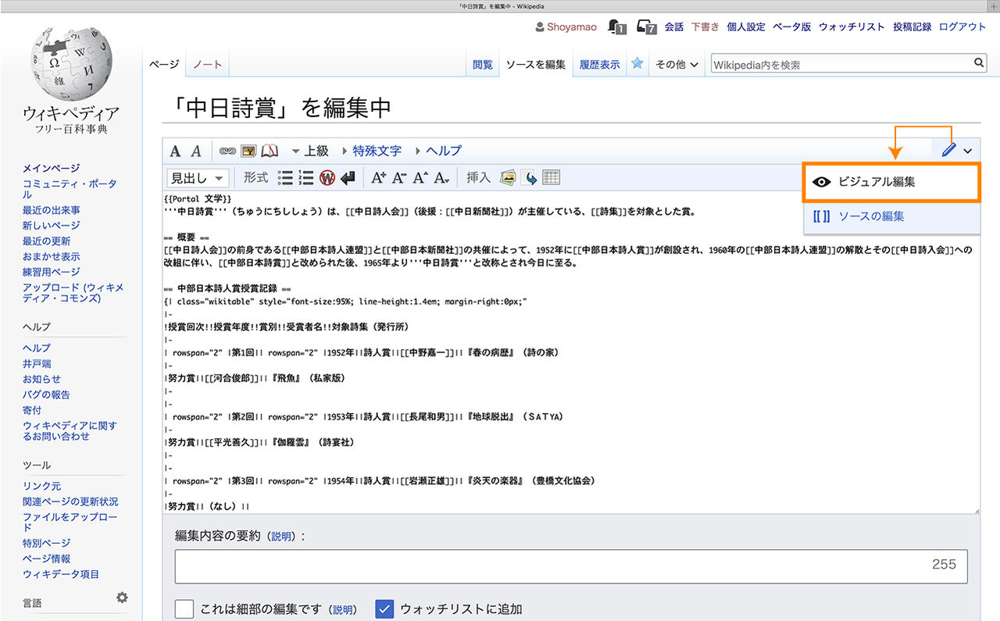
\includegraphics[width=120mm]{images/wikipedia_edit.png}
  \caption{Wikipediaでの編集画面} \label{fig:wikipedia_edit}
\end{figure}

\subsection{NFC技術とWikiの併用}
上記のようなNFC技術とWikiの利点を組み合わせることで要件5も満たすことができる。

\subsubsection*{要件5:広い分野の知見と用途を総合的に管理できる}
Wikiはハイパーリンクで情報を整理・参照するため、グループによる情報分類や階層的な情報の管理を必要としない。
したがってWikiでは異なる分野の情報をフラットに管理し、参照することができる。
実際ににWikiシステムを利用した百科事典であるWikipediaはあらゆる分野の情報を総合的に管理しながらも破綻なくシステムを運用している。
このようなWikiシステムをAR情報の管理に利用することで、分野を横断した知見の管理が可能になり、様々な用途に対応したナビゲーションシステムを作成できる。

Wikiシステムを利用すると広い分野の情報を一元的に管理することができるが、一方で自身の欲しい情報を探す際に手間となる事がある。
これを避けるためにNFCタグに記録されたコンテキスト情報を活用しフィルタが可能なシステムを本研究では採用した。
位置情報だけでなくNFCタグに登録された、情報源とするWikiプロジェクトや特定のリンクを元にユーザ側から見える情報をフィルタすることができる。
これより広い分野の情報を一元的に管理できるWikiの利点を活かしながら様々な用途に対応したナビゲーションを提供する事が可能になる.



\section{まとめ}
本章では第\ref{chap:background}章で整理したARナビゲーションの現状と問題点を元に次世代ARナビゲーションシステム、HypAR Touchの要件を定義した。
さらに定義した要件はNFC技術とWikiシステムを組み合わせることで達成されることを提案し、その詳細を設計で示した。
次章では本設計を元に開発したHypAR Touchの実装とその機能を説明する。



% 以下以前の章立てでの記述(移行済み)


% \section{HypAR Touch}
% 本研究で提案するARナビゲーションシステムであるHypAR Touchの基本構成と使い方を解説する。

% \subsection{基本構成}
% 本研究で提案するARナビゲーションシステムHypAR Touchはモバイル端末向けアプリケーションであるHypAR Touch アプリと専用のNFCタグ、WikiであるScrapboxで構成されている。

% \paragraph*{HypAR Touchアプリ} 
% HypAR TouchアプリはARでのナビゲーションを表示するモバイル端末向けネイティブアプリケーションである。
% 後述する専用のNFCタグにタッチすることでARナビゲーションを表示することができる。
% NFCタグの読み取り機能を持つAndroid\footnote{\textsf{https://www.android.com/}}端末とiOS\footnote{\textsf{https://www.apple.com/jp/ios}}端末に対応しており、現在流通する多くのモバイル端末で利用可能である。

% \paragraph*{NFCタグ}
% 本システムではモバイル端末の位置情報測位および提示するナビゲーションの出し分けのためにNFCタグを利用している。
% NFCタグにはISO/IEC 14443のTypeA\footnote{\textsf{https://www.nxp.com/docs/en/application-note/AN10834.pdf}}規格に準拠するNFCタグを利用しており、NDEF\footnote{\textsf{https://nfc-forum.org/our-work/specification-releases/specifications/nfc-forum-technical-specifications/}}(NFC Data Exchange Format)形式で情報を記録している。
% このタグタイプと情報形式はNFC機能を持つほとんどのモバイル端末で読み取りがサポートされており、アプリを起動していない状態でのバックグラウンド読み取りにも対応している。
% さらにタグ内に記録する情報としてCustomURLSchemeを利用することでアプリが起動していない状態でもNFCタグにタッチすることでHypAR Touchアプリの起動を可能としている。

% \paragraph*{Scrapbox}
% Scrapbox(図\ref{fig:scrapbox})はGyazz\cite{Gyazz}をベースにして開発された、Nota\footnote{\textsf{https://www.notainc.com/ja}}社が運営しているWikiである。
% 本システムではこのScrapboxをARで表示する情報の管理ツールとして利用している。
% これはScrapboxが他のシステムには存在しない以下のようなHypAR Touchに適した特徴を持つためである。
% \begin{itemize}
%   \item シンプルで柔軟な記法をもつWYSIWYGエディタ
  
%   入力/改行/段落/箇条書きといった基本的なテキスト編集を見たまま行える。
  
%   \item 場所指定に最適なLocation記法
  
%   Google MapsのURLを貼り付けるだけで地図を埋め込めるLocation記法\footnote{\textsf{https://scrapbox.io/help-jp/Location記法}}と呼ばれる機能があり地理情報を記述するのに適している。
%   本システムではこのLocation記法によって表示する情報の場所を指定している。

%   \item リンク記法によるシンプルなハイパーリンクと関連ページリスト
  
%   Scrapboxでは単語を\texttt{[]}で囲うだけで同一wiki内ページへのリンクとすることが可能である。
%   さらにScrapboxページの下部には
%   \begin{itemize}
%       \item 別ページへのリンク
%       \item 別ページからのリンク
%       \item リンク先ページがリンクしているページ
%   \end{itemize}
%   といった関連ページリスト(図\ref{fig:scrapbox_related})が表示され、どのような情報と関連するのかが一目瞭然に分かる。

% \end{itemize}

% \begin{figure}[h]
%   \begin{minipage}{0.5\hsize}
%     \centering
%     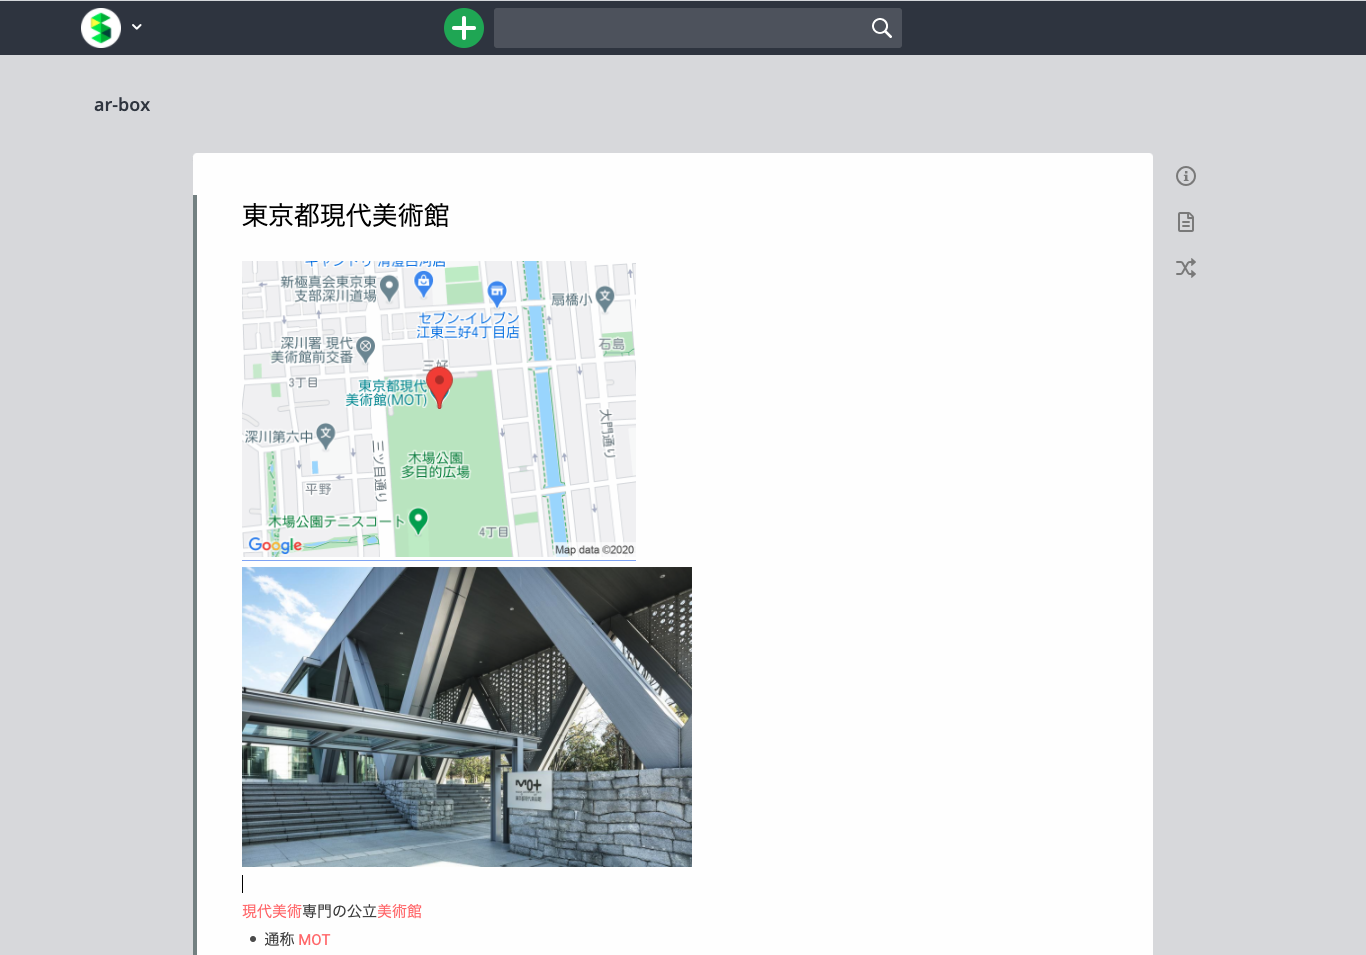
\includegraphics[width=75mm]{images/scrapbox_screen.png}
%     \caption{Scrapboxの画面} \label{fig:scrapbox}
%   \end{minipage}
%   \begin{minipage}{0.5\hsize}
%     \centering
%     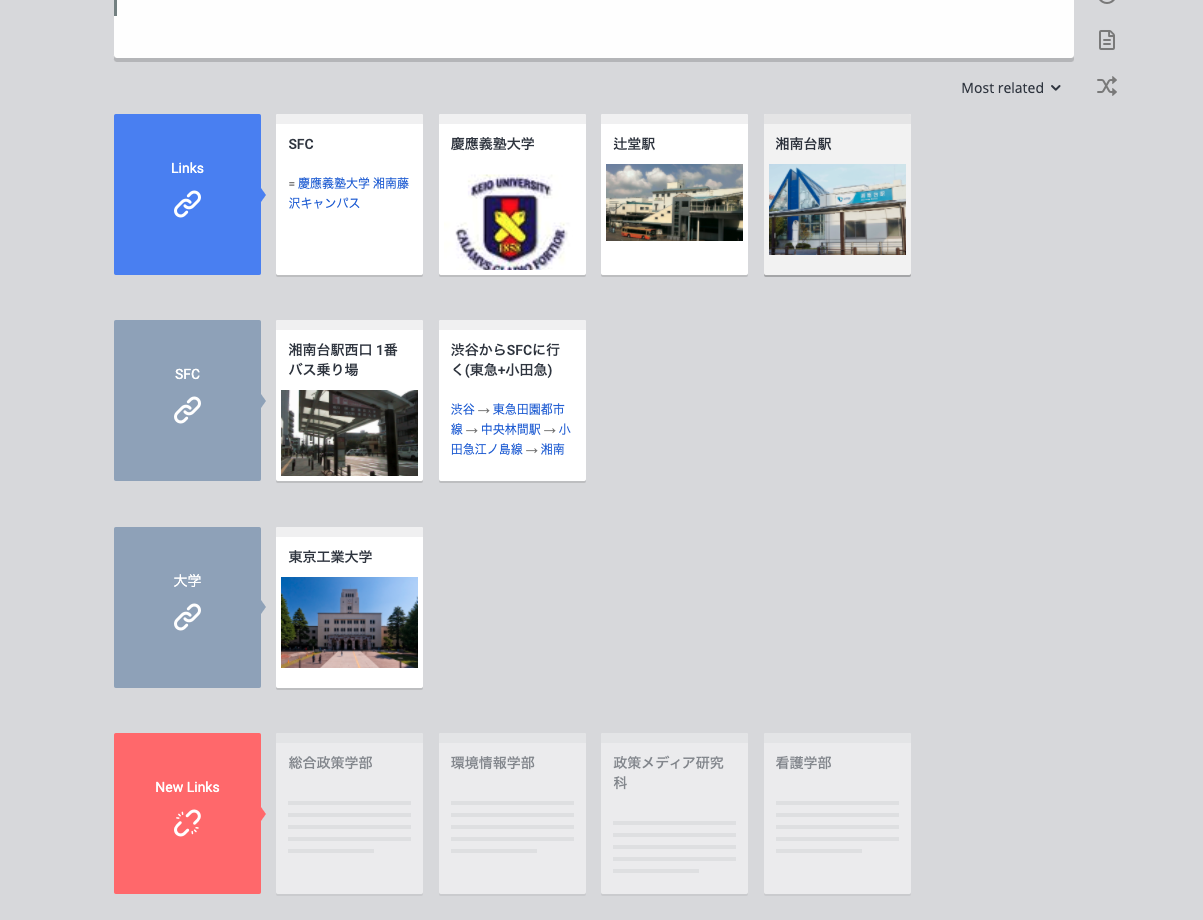
\includegraphics[width=75mm]{images/scrapbox_related_screen.png}
%     \caption{Scrapboxの関連ページリスト} \label{fig:scrapbox_related}
%   \end{minipage}
% \end{figure}


% \subsection{使い方}

% \subsubsection{HypAR Touchアプリによるナビゲーション閲覧}
% \paragraph*{NFCタグにタッチする}
% 本アプリケーションは図\ref{fig:touch_nfc}のように専用の情報が書かれたNFCタグにタッチすることで起動し、ナビゲーションを開始する。
% NFCにタッチすることで端末の位置と向きが認識され、図\ref{fig:hypar_touch_init_screen}のように登録された情報をARで正しい位置に表示することができる。
% また画面下部にあるスライダー(図\ref{fig:hypar_touch_slider})を動かすことでARで表示する情報の距離の範囲を指定することができる。

% \begin{figure}[h]
%   \centering
%   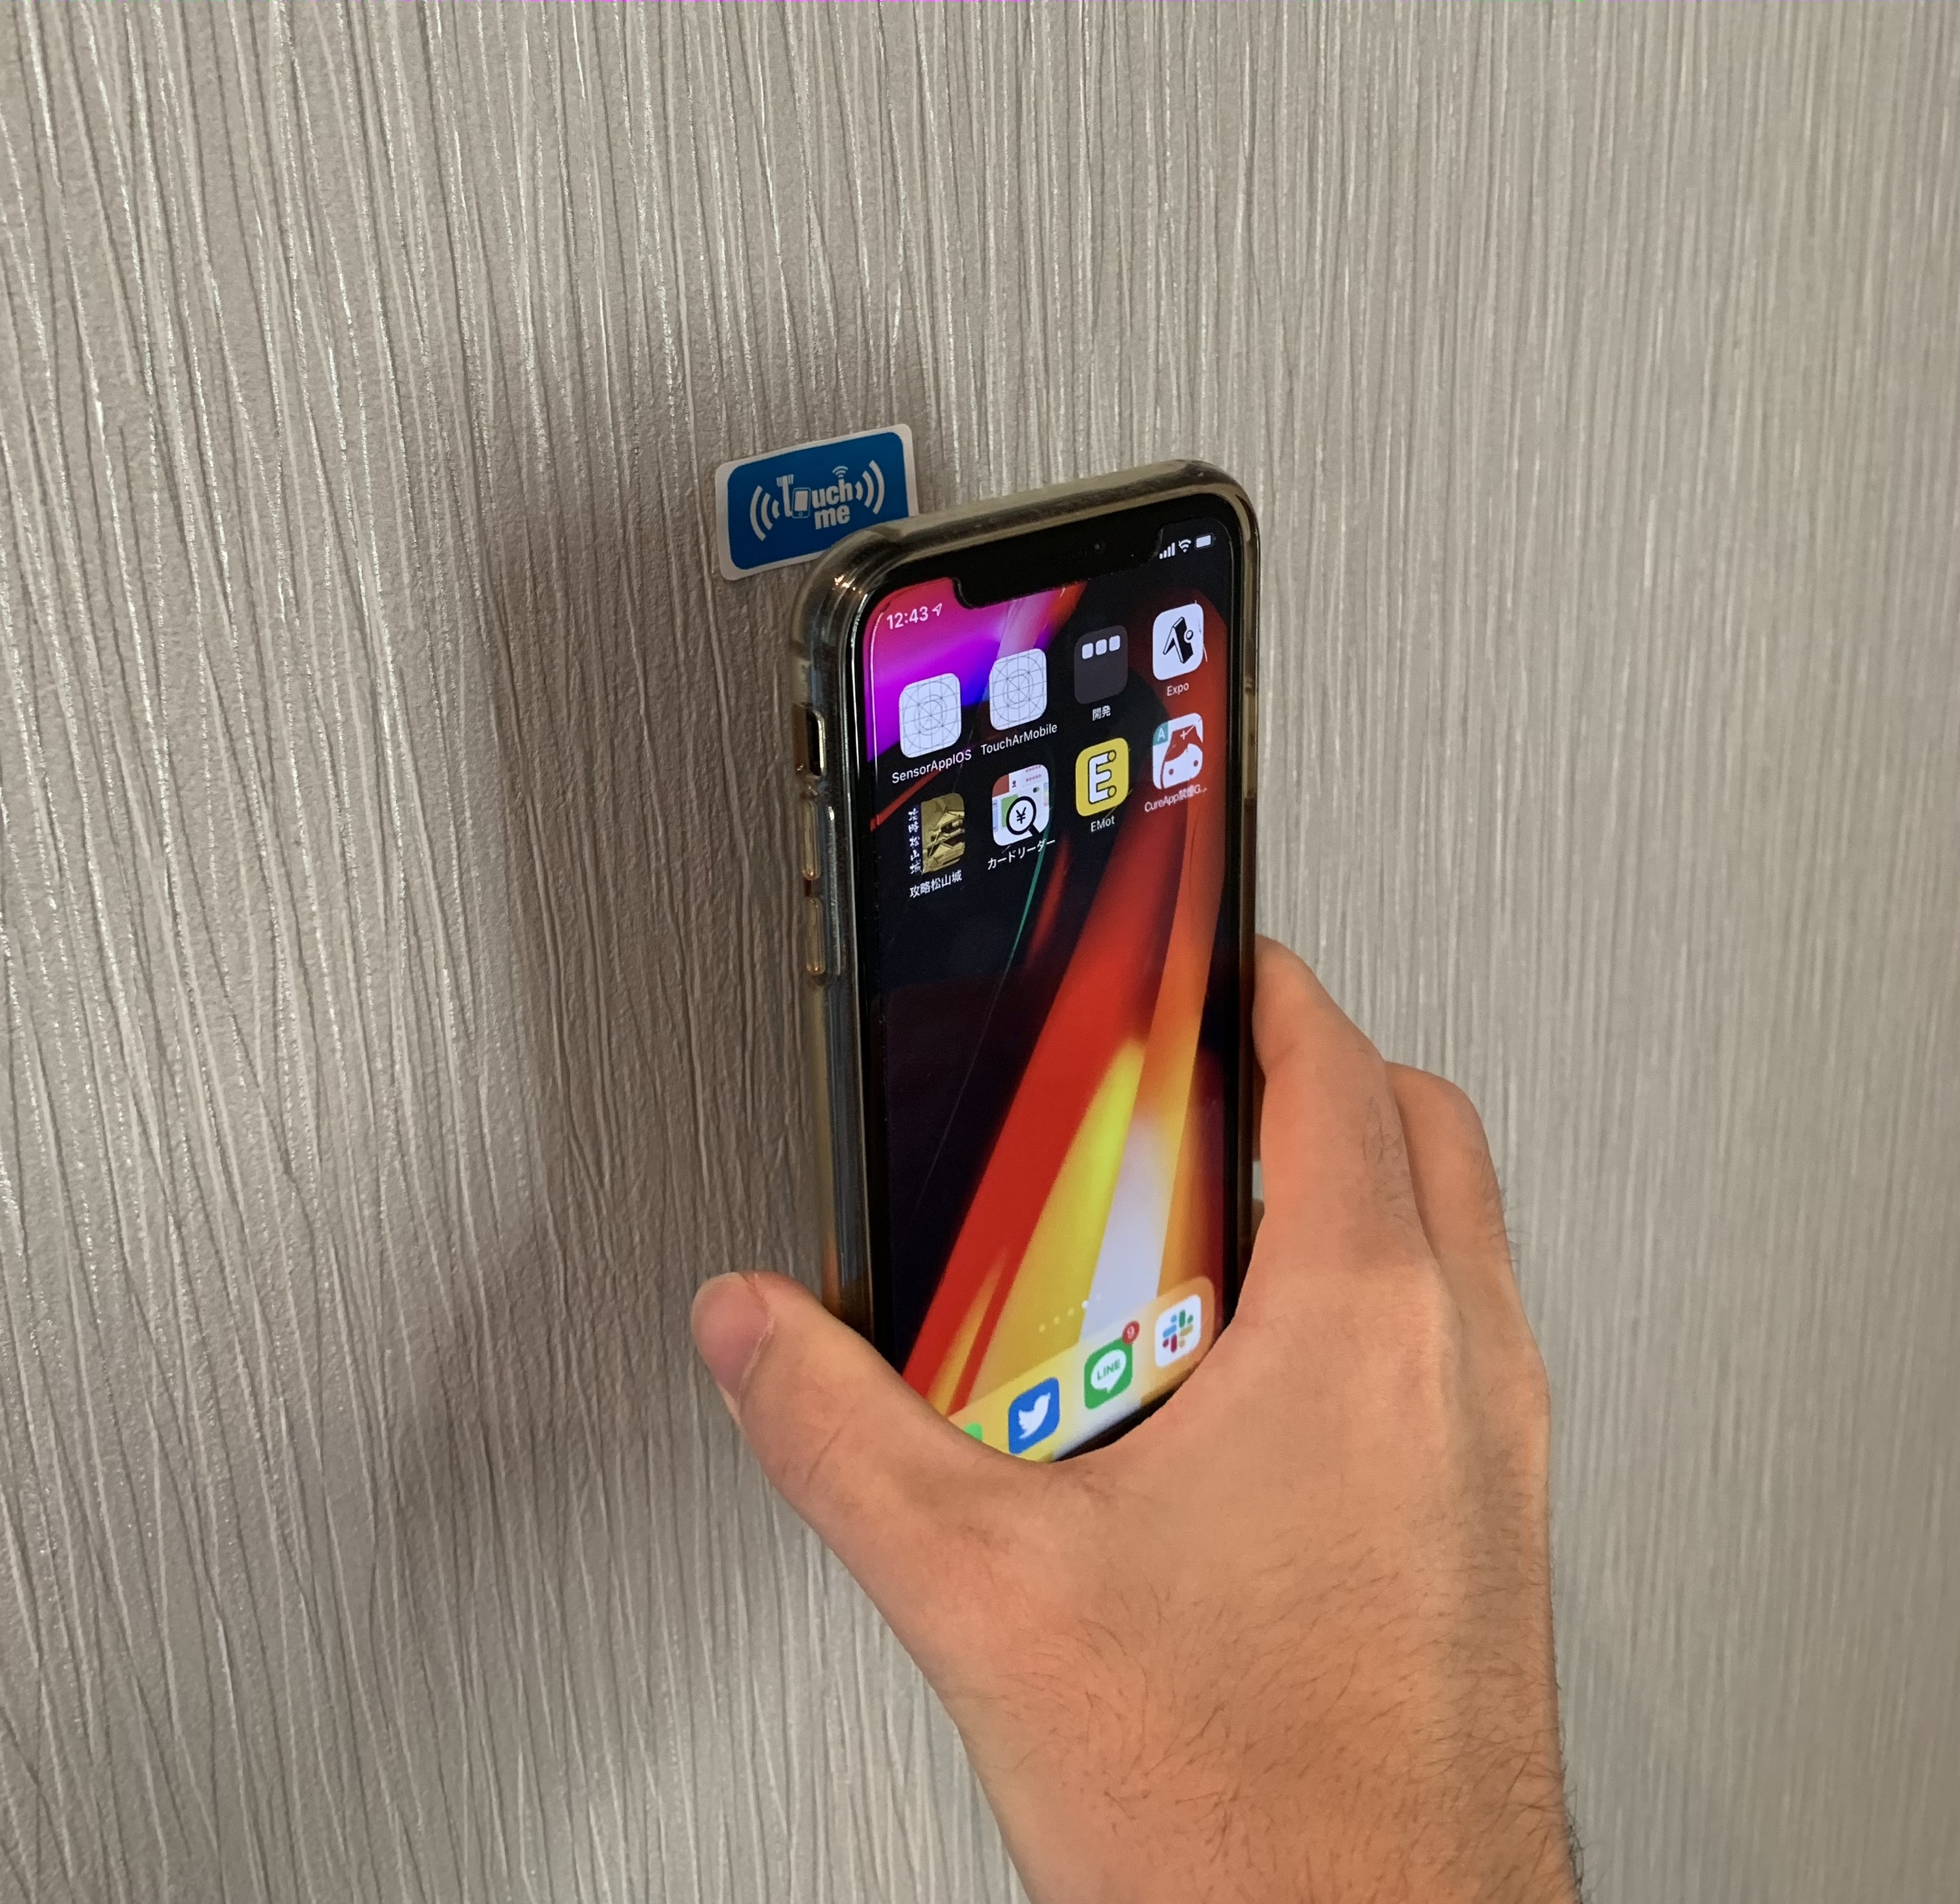
\includegraphics[width=100mm]{images/touch_nfc.jpg}
%   \caption{NFCタグにタッチする様子} \label{fig:touch_nfc}
% \end{figure}

% \begin{figure}[h]
%   \begin{minipage}{0.5\hsize}
%     \centering
%     \includegraphics[height=100mm]{images/hypar_touch_init_screen.png}
%     \caption{ARでの表示} \label{fig:hypar_touch_init_screen}
%   \end{minipage}
%   \begin{minipage}{0.5\hsize}
%     \centering
%     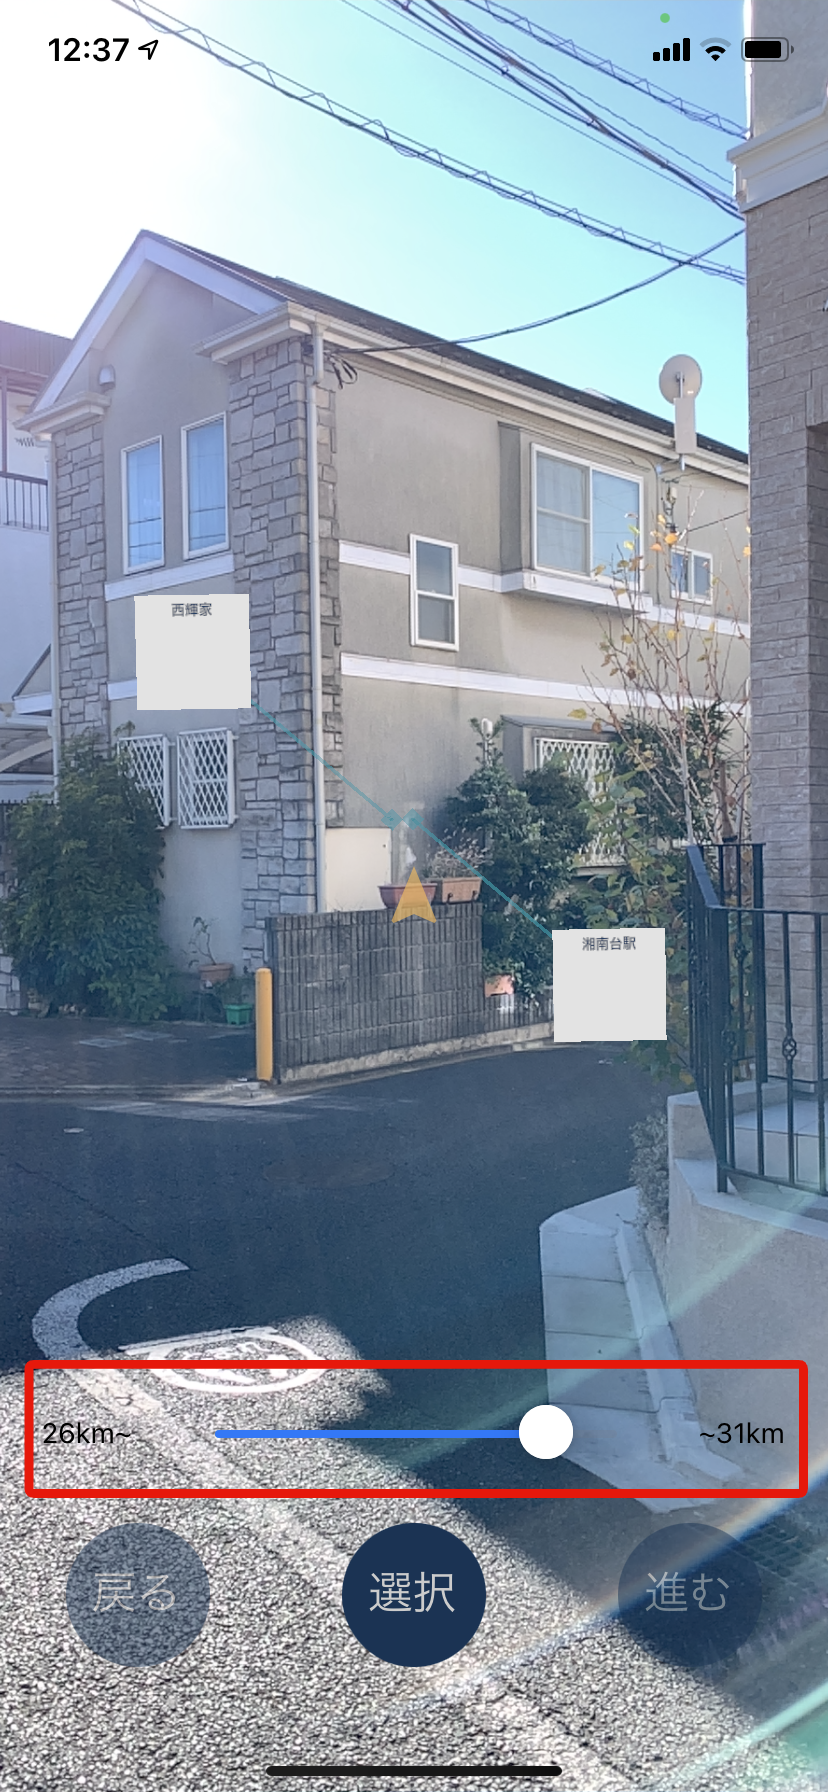
\includegraphics[height=100mm]{images/hypar_touch_slider.png}
%     \caption{スライダーによる距離指定} \label{fig:hypar_touch_slider}
%   \end{minipage}
% \end{figure}

% \paragraph*{表示されたAR情報の関連情報を表示・選択する}
% 画面の中央にはオレンジ色の三角のカーソルが表示されており、これをARで表示された情報の上に重ねると青い枠線が表示される(図\ref{fig:hypar_touch_hover})。
% その状態で画面下部の選択ボタンを押すと図\ref{fig:hypar_touch_selected}のように関連する情報が放射状に配置されてに表示される。
% これらの表示された関連情報も同じようにカーソルで選択することができる(図\ref{fig:hypar_touch_sub_selected})。
% このように関連情報を選択していくことによって興味のある情報をAR上で探索することができる。

% \begin{figure}[h]
%   \begin{minipage}{0.5\hsize}
%     \centering
%     \includegraphics[height=100mm]{images/hypar_touch_hover.png}
%     \caption{カーソルを重ねた状態} \label{fig:hypar_touch_hover}
%   \end{minipage}
%   \begin{minipage}{0.5\hsize}
%     \centering
%     \includegraphics[height=100mm]{images/hypar_touch_selected.png}
%     \caption{選択した状態} \label{fig:hypar_touch_selected}
%   \end{minipage}
% \end{figure}

% \begin{figure}[h]
%     \centering
%     \includegraphics[height=100mm]{images/hypar_touch_sub_selected.png}
%     \caption{関連情報の選択} \label{fig:hypar_touch_sub_selected}
% \end{figure}


% \paragraph*{選択されたAR情報の詳細を見る}
% 上記のようにカーソルをAR情報にあわせた上で選択ボタンを押すと画面上部には図\ref{fig:hypar_touch_top}のように選択された情報のタイトルの他に「see more」と書かれたボタンが出現する。
% これをクリックすることでAR情報の元となったScrapboxをみることが可能である(図\ref{fig:hypar_touch_webview})。

% \begin{figure}[h]
%   \begin{minipage}{0.5\hsize}
%     \centering
%     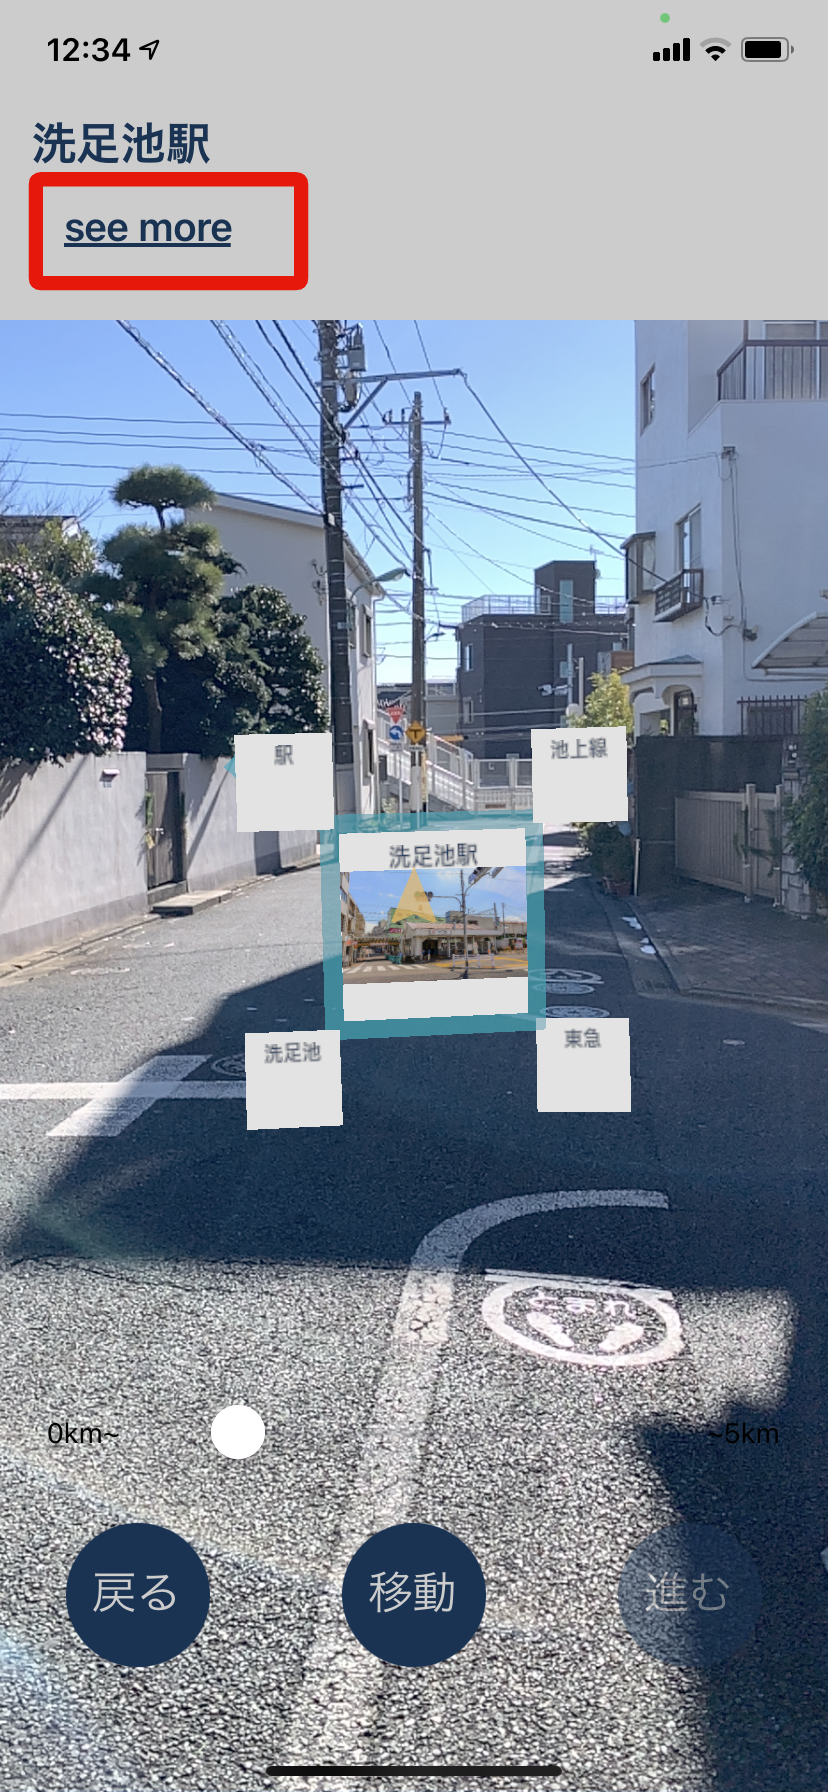
\includegraphics[height=100mm]{images/hypar_touch_top.png}
%     \caption{詳細を表示するボタン} \label{fig:hypar_touch_top}
%   \end{minipage}
%   \begin{minipage}{0.5\hsize}
%     \centering
%     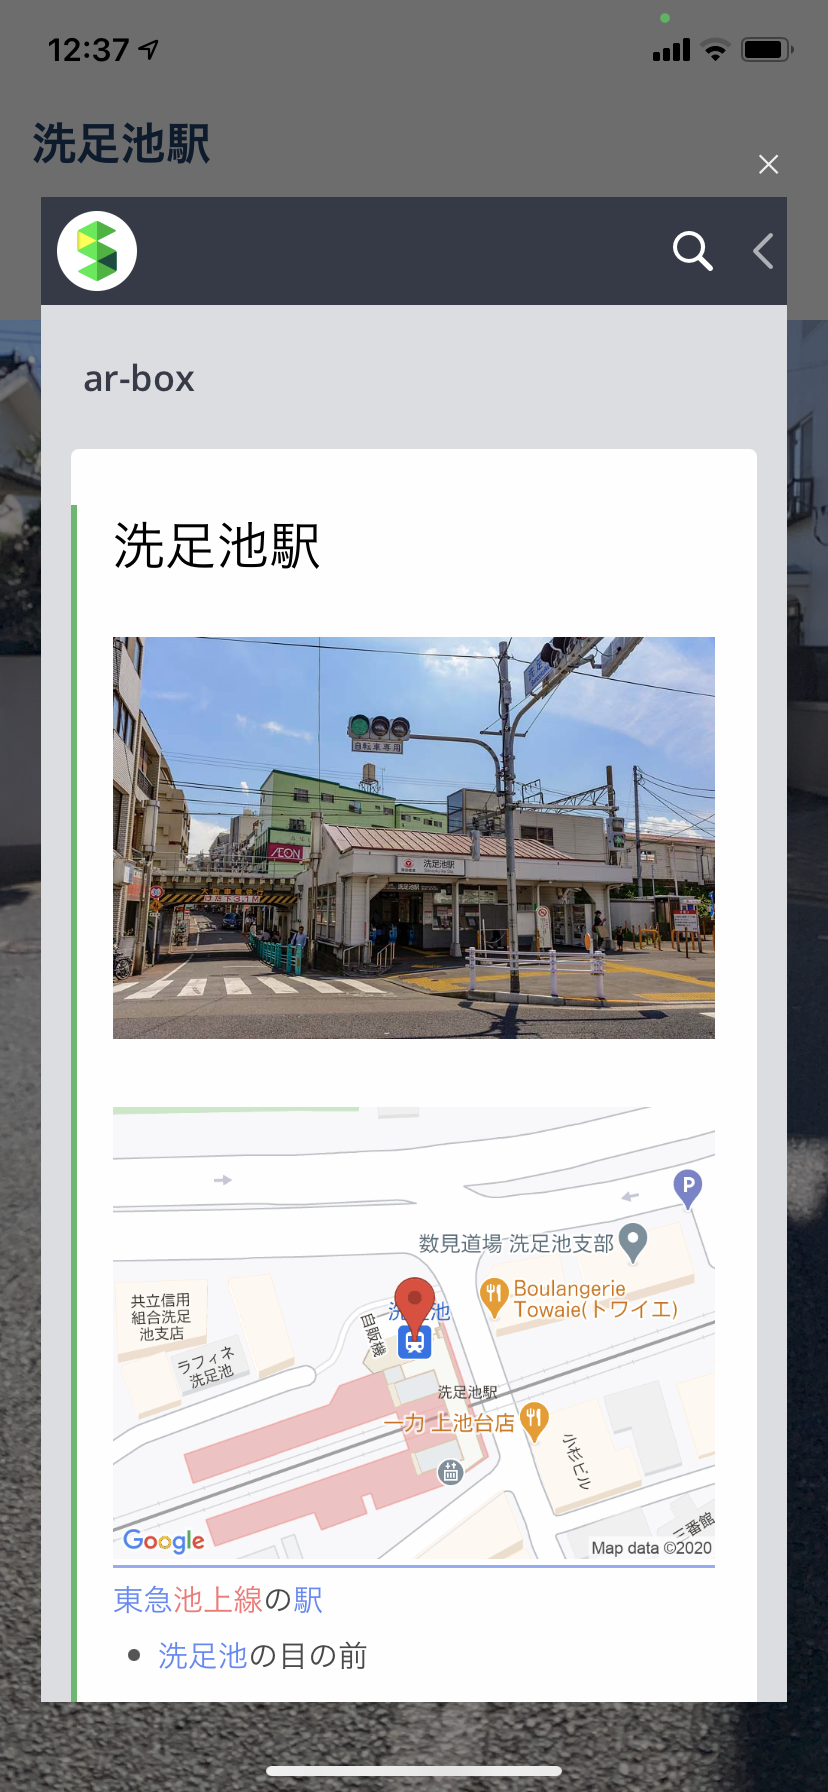
\includegraphics[height=100mm]{images/hypar_touch_webview.png}
%     \caption{Scrapboxでの情報表示} \label{fig:hypar_touch_webview}
%   \end{minipage}
% \end{figure}

% \paragraph*{選択されたAR情報の場所に視点を移動する}
% 同じようにカーソルをAR情報にあわせた上で選択ボタンを押し、もう一度選択したAR情報にカーソルを重ねると画面下部中央のボタンが「移動」に変化する(図\ref{fig:hypar_touch_move_button})
% この移動ボタンを押すと図\ref{fig:hypar_touch_move_map}のような地図での移動アニメーションを経て、選択した情報のある場所からの視点(図\ref{fig:hypar_touch_moved})に切り替えることができる。

% \begin{figure}[h]
%   \begin{minipage}{0.5\hsize}
%     \centering
%     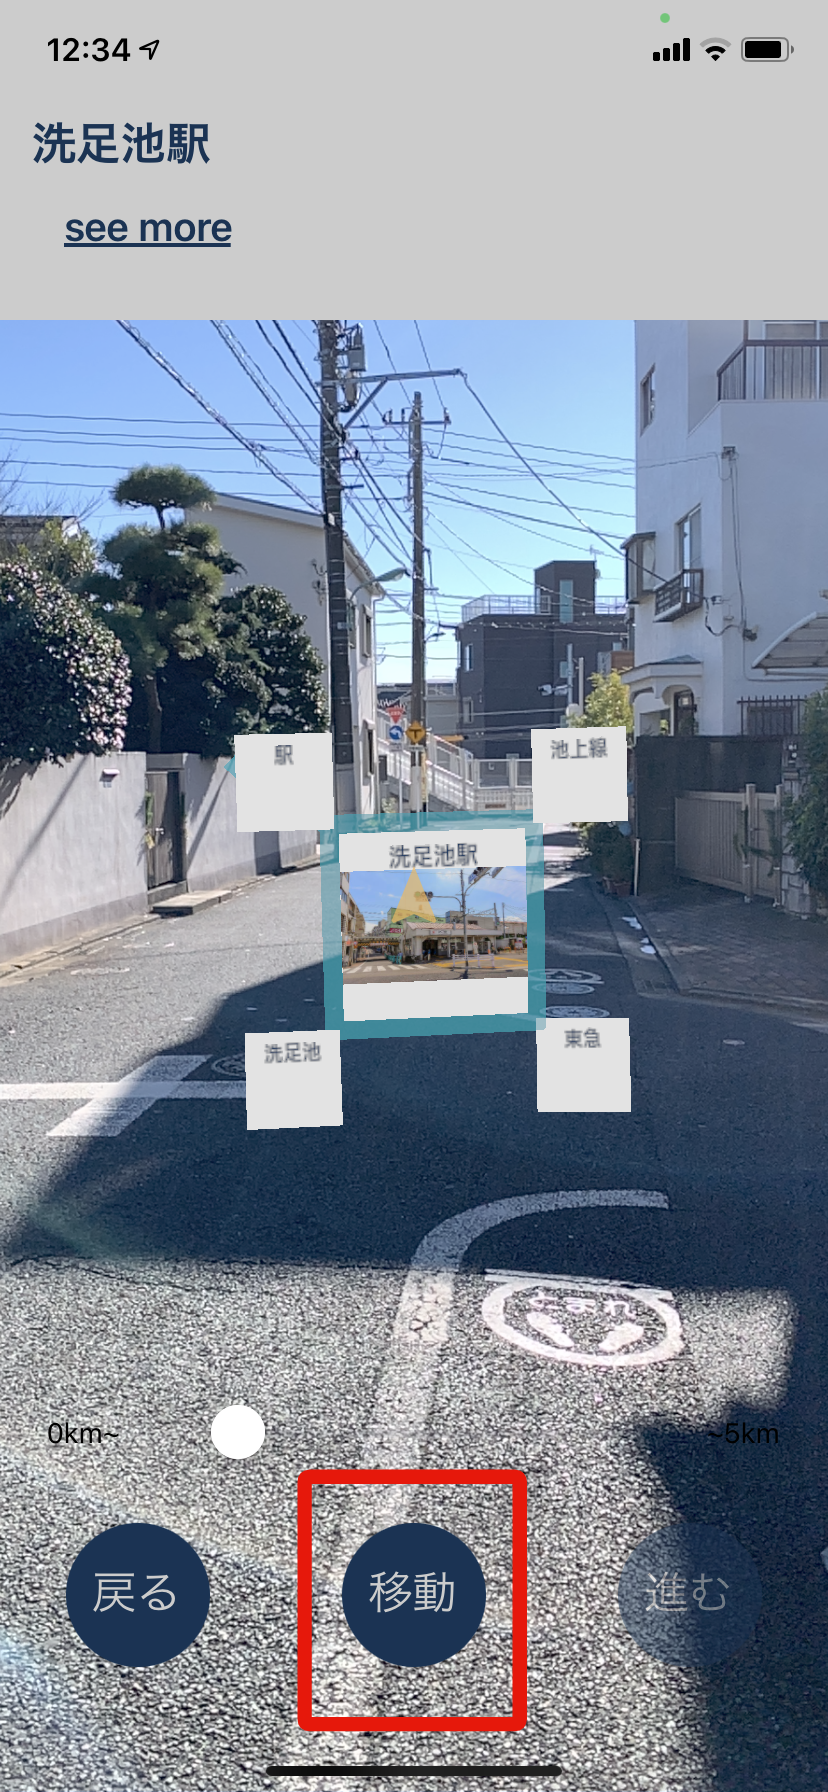
\includegraphics[height=100mm]{images/hypar_touch_move_button.png}
%     \caption{移動ボタン} \label{fig:hypar_touch_move_button}
%   \end{minipage}
%   \begin{minipage}{0.5\hsize}
%     \centering
%     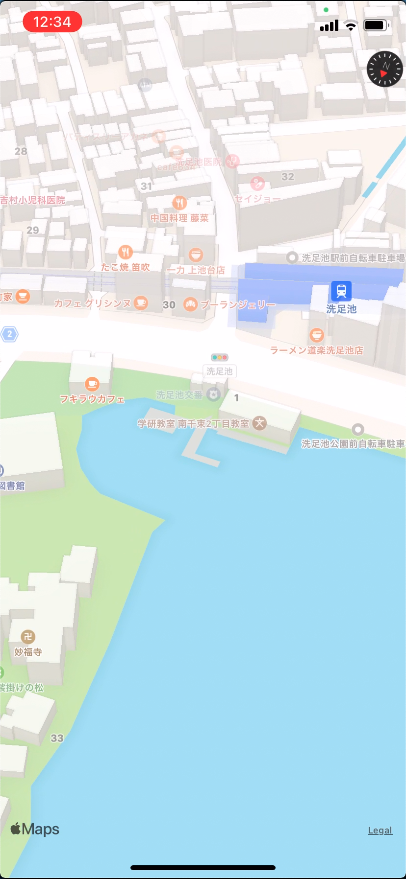
\includegraphics[height=100mm]{images/hypar_touch_move_map.png}
%     \caption{Mapでの移動アニメーションの途中} \label{fig:hypar_touch_move_map}
%   \end{minipage}
% \end{figure}

% \begin{figure}[h]
%   \centering
%   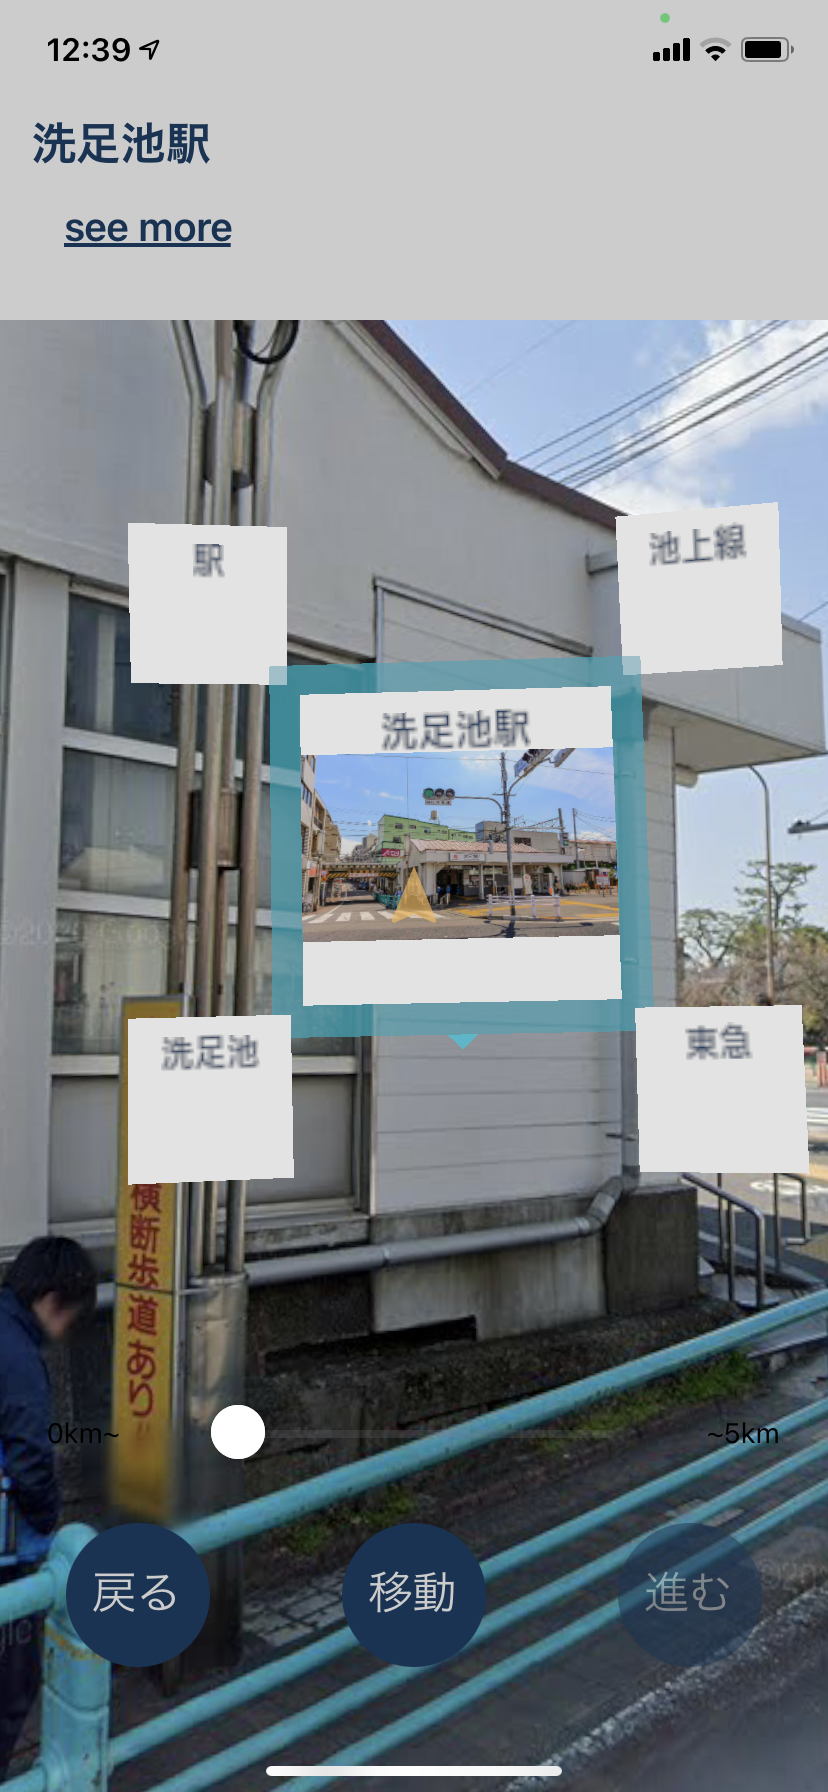
\includegraphics[height=100mm]{images/hypar_touch_moved.png}
%   \caption{移動先からの視点} \label{fig:hypar_touch_moved}
% \end{figure}

% \paragraph*{AR情報の選択を解除する・前の状態に戻る}
% 上記のような選択状態は画面の何も表示されていない部分をタップすることで解除できる。
% また選択や移動した履歴情報は常に保存されており、画面下部の「戻る」「進む」ボタン(図\ref{fig:hypar_touch_history_button})で履歴を参照することができる。

% \begin{figure}[h]
%   \centering
%   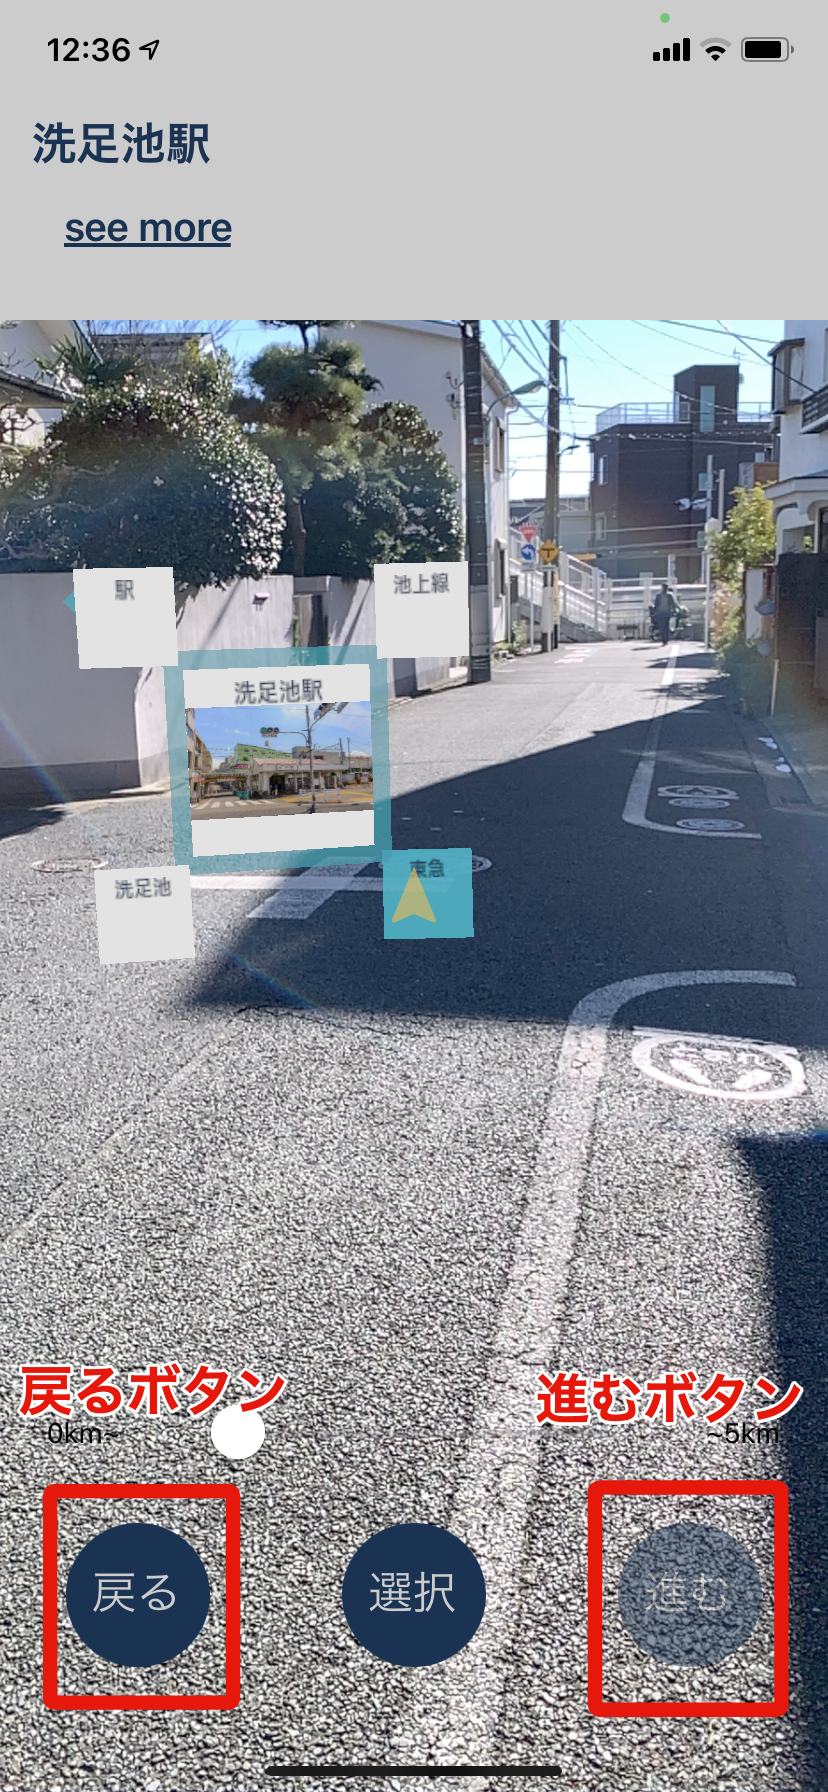
\includegraphics[width=70mm]{images/hypar_touch_history_button.png}
%   \caption{進むボタンと戻るボタン} \label{fig:hypar_touch_history_button}
% \end{figure}

% \subsubsection{ScrapboxによるAR情報法の追加・編集}
% HypAR Touchアプリに表示されるAR情報はNFCタグで指定されたScrapboxのプロジェクトをもとに生成される。
% Scrapboxのプロジェクトにあるページのうち、Location記法によって位置情報の記述のあるページがアプリ側で表示されるAR情報と対応する。

% \paragraph*{ARで表示する情報を追加する}
% AR情報はScrapboxのページと対応しているため、新しくページを作成し、以下の2点の情報を記入することでAR情報が登録される。
% \begin{itemize}
%   \item ページタイトル
  
%   図\ref{fig:scrapbox_ar_new}の\textcircled{\scriptsize{1}}部分であり、ページを作る上で必須となる項目である。
%   このタイトルはHypAR Touchアプリ側でサムネイルとともにAR表示される。

%   \item Location記法による記述
  
%   Scrapboxにはソースコード \ref{google_map_url}のようなGoogle MapsのURLをソースコード \ref{location}のようなLocation記法に変換し、図\ref{fig:scrapbox_ar_new}の\textcircled{\scriptsize{2}}のようにマップとして表示する機能がある。
%   この機能を利用し、AR情報を追加したい場所を中心としたGoogleMapのURLをScrapboxに貼り付けることでAR上で表示する場所を指定する。

%   \begin{lstlisting}[caption=googleMapのURL, label=google_map_url]
%     https://www.google.com/maps/place/%E6%9D%B1%E4%BA%AC%E9%A7%85/@35.681502,139.7671784,17z/data=!4m5!3m4!1s0x60188bfbd89f700b:0x277c49ba34ed38!8m2!3d35.6812362!4d139.7671248
%   \end{lstlisting}

%   \begin{lstlisting}[caption=Location記法, label=location]
%     [N35.681502,E139.7671784,Z16 東京駅]
%   \end{lstlisting}
% \end{itemize}

% \begin{figure}[h]
%   \centering
%   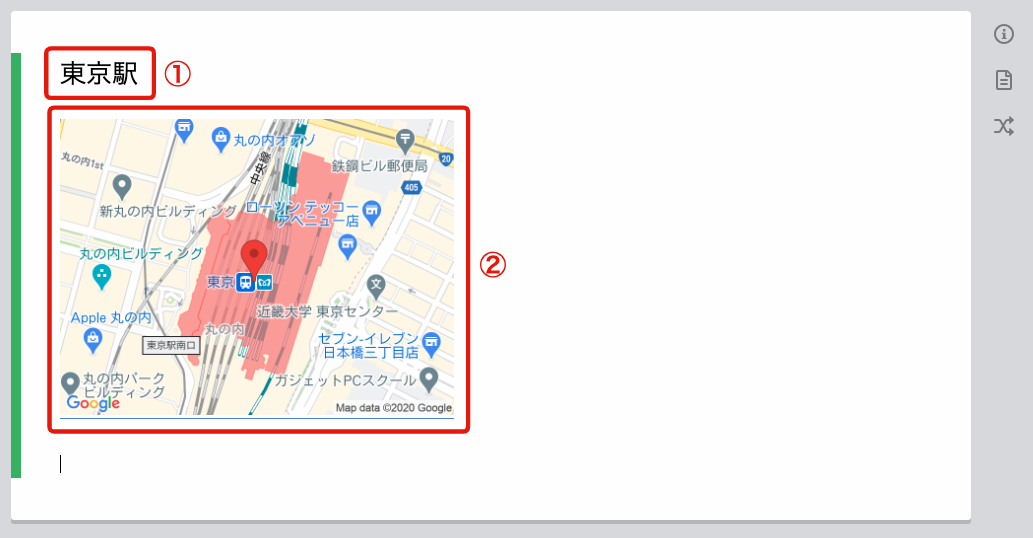
\includegraphics[width=120mm]{images/scrapbox_ar_new.png}
%   \caption{新しくページを作成した時} \label{fig:scrapbox_ar_new}
% \end{figure}

% \paragraph*{サムネイルを追加する}
% Scrapboxでは画像のURLを\texttt{[]}で囲う、または画像をドラッグ・アンド・ドロップすることで図\ref{fig:scrapbox_thumbnail}のようにページに画像を表示させることができる。
% このようにScrapboxのページに画像を貼ると、ページの一番上にある画像がAR表示でのサムネイルになる。(図\ref{fig:scrapbox_thumbnail_and_ar})

% \begin{figure}[h]
%   \centering
%   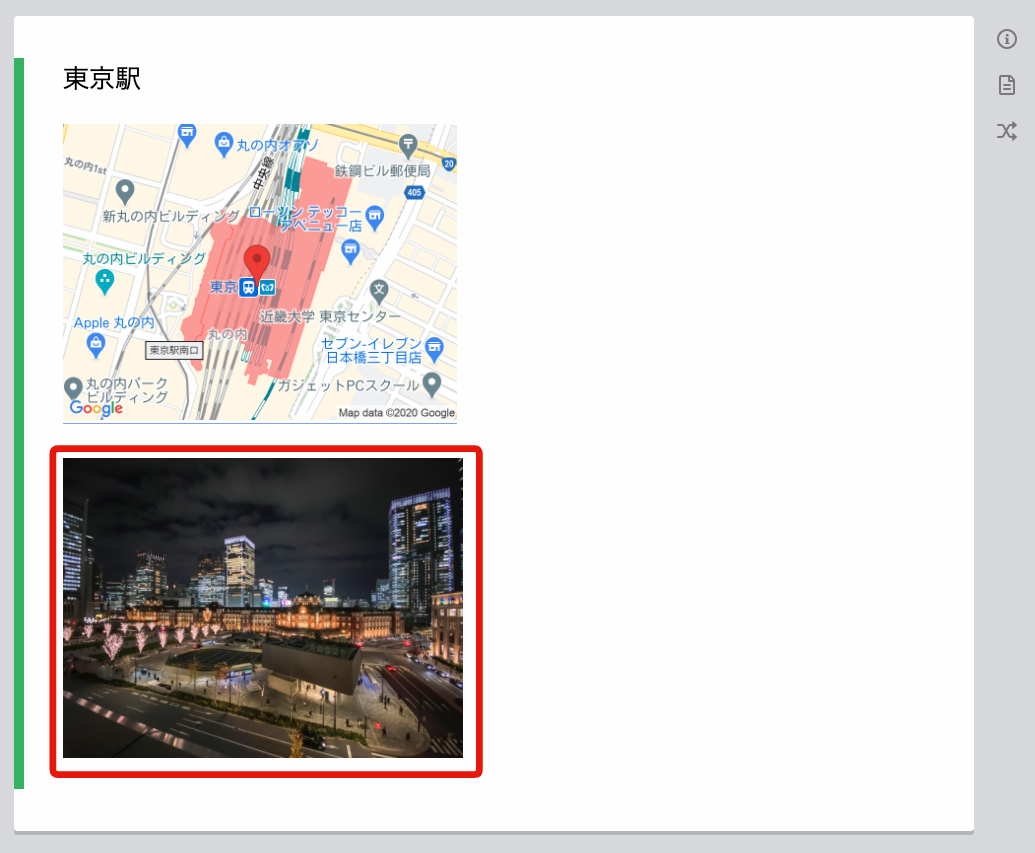
\includegraphics[width=120mm]{images/scrapbox_thumbnail.png}
%   \caption{Scrapboxに貼り付けた画像} \label{fig:scrapbox_thumbnail}
% \end{figure}

% \begin{figure}[h]
%   \centering
%   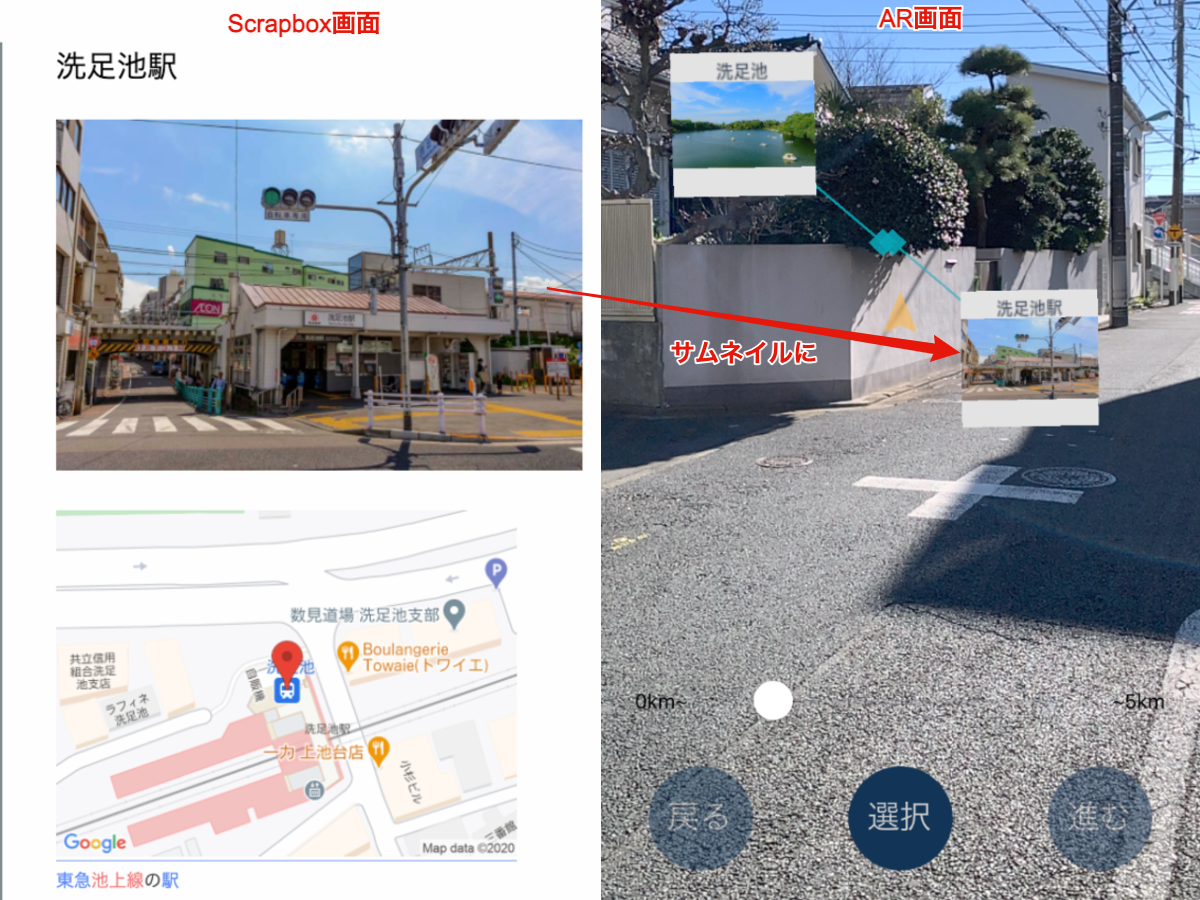
\includegraphics[width=120mm]{images/scrapbox_thumbnail_and_ar.png}
%   \caption{Scrapbox上の画像とARでの表示} \label{fig:scrapbox_thumbnail_and_ar}
% \end{figure}

% \paragraph*{ハイパーリンクを利用して説明を書く}
% Scrapboxでは単語を\texttt{[]}で囲うことにより同一wiki内ページへのハイパーリンクとすることが可能である。
% 他ページヘのハイパーリンクが生成されるとAR上で関連情報として表示されるようになる(図\ref{fig:scrapbox_link_and_ar})。
% ARで表示したい情報の説明を書き、説明文中の単語を積極的にハイパーリンクにすることで関連する情報を提示することができる。

% \begin{figure}[h]
%   \centering
%   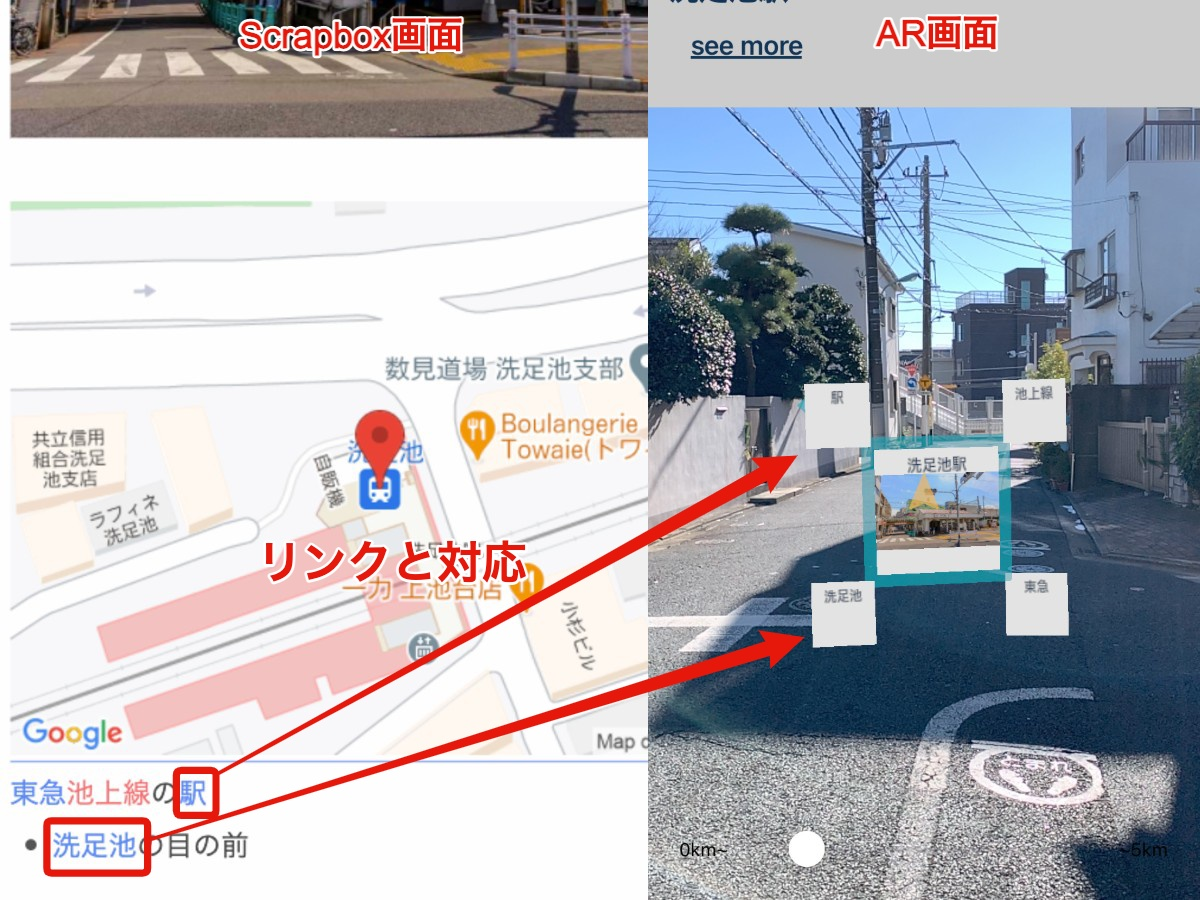
\includegraphics[width=120mm]{images/scrapbox_link_and_ar.jpg}
%   \caption{Scrapbox上のリンクとARでの表示} \label{fig:scrapbox_link_and_ar}
% \end{figure}

% \subsubsection{NFCタグに対する情報の書き込み}
% NFCタグにはISO/IEC 14443 TypeAに準拠したNTAGを利用する。
% また情報を記録する際にはNFC FORUM\footnote{\textsf{https://nfc-forum.org}}によって標準化されているNDEFフォーマットで情報を書き込む。
% 書き込む情報は図\ref{fig:nfc_uri}のようにCustomURLSchemeに沿ったURIの形式で書き込む。

% \begin{figure}[h]
%   \centering
%   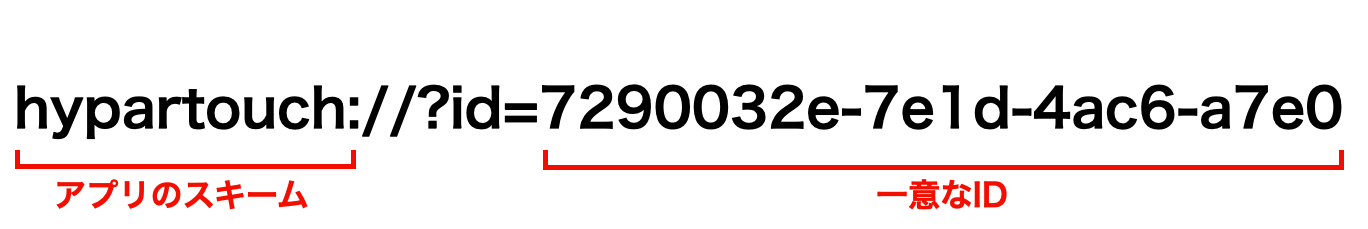
\includegraphics[width=120mm]{images/nfc_uri.png}
%   \caption{NFCに書き込むURIデータ} \label{fig:nfc_uri}
% \end{figure}

% その上でタグに書き込んだIDと紐付ける形でHypAR Touchのサーバーに以下の情報を登録する。
% \begin{itemize}
%   \item 緯度経度
%   \item タグの設置される向き(0〜360度)
%   \item 表示するAR情報の元となるScrapboxのプロジェクト
%   \item タッチした時に選択されているリンク情報
% \end{itemize}
% これらの情報はHypAR Touchアプリ内の登録画面(図\ref{fig:nfc_register_mobile})により登録可能である。

% \begin{figure}[h]
%   \centering
%   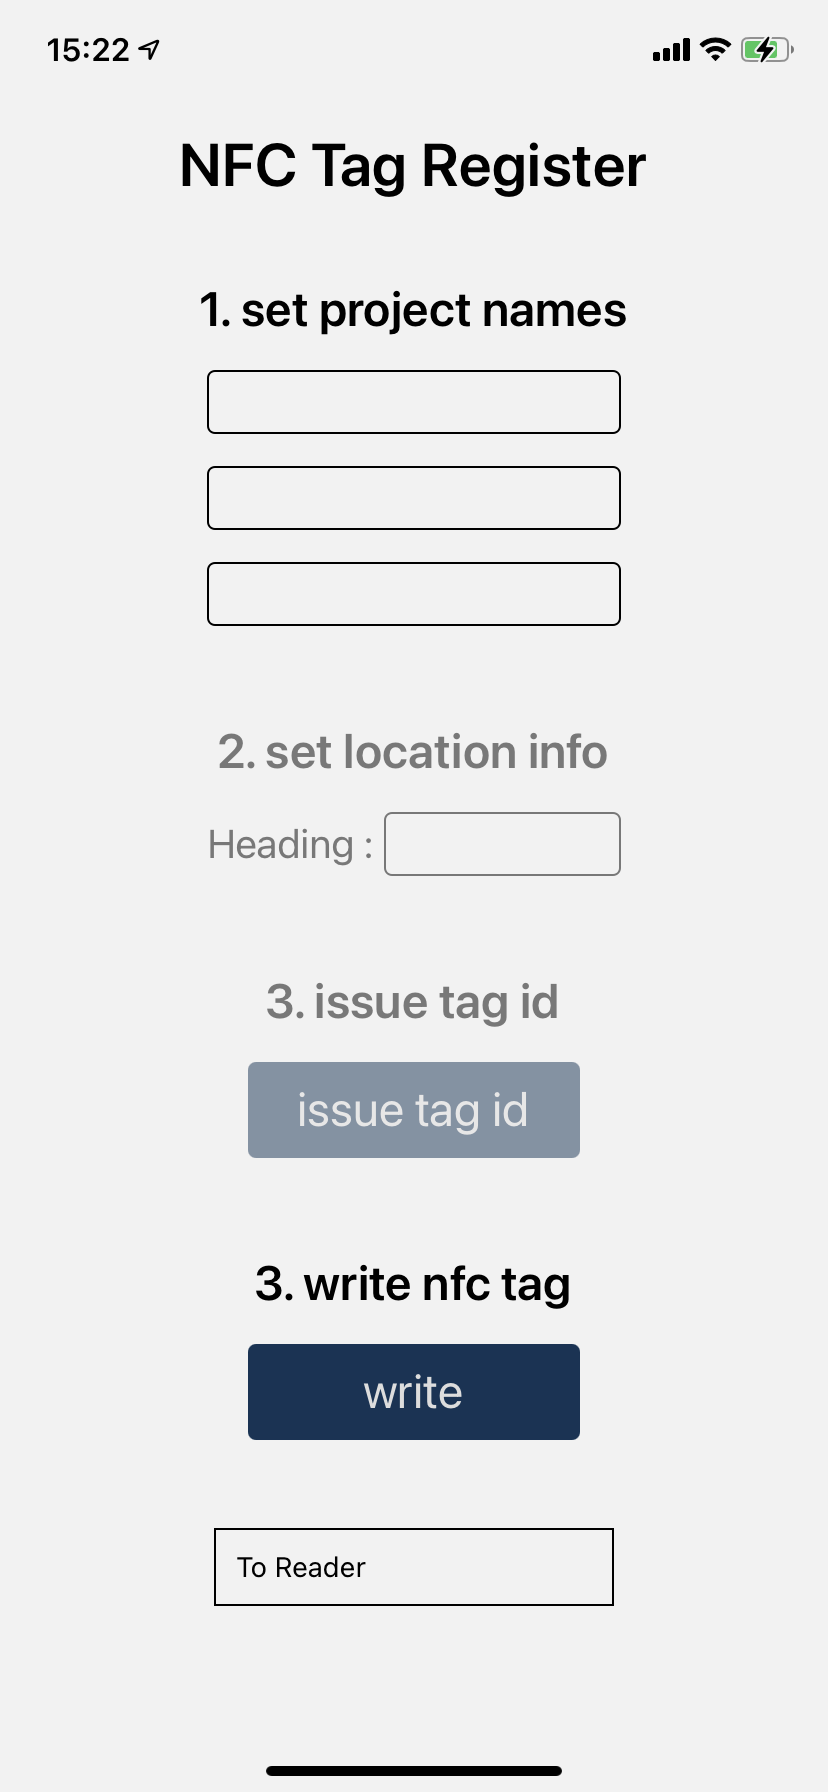
\includegraphics[width=70mm]{images/nfc_register_mobile.png}
%   \caption{モバイルアプリでの登録} \label{fig:nfc_register_mobile}
% \end{figure}